% Meta-Informationen -------------------------------------------------------
%		Informationen über das Dokument, wie z.B. Titel, Autor, Matrikelnr. etc
%		werden in der Datei _Meta.tex definiert und können danach global
%		verwendet werden.
% --------------------------------------------------------------------------
% Informationen ------------------------------------------------------------
% 	Definition von globalen Parametern, die im gesamten Dokument verwendet
% 	werden können (z.B auf dem Deckblatt etc.).
% --------------------------------------------------------------------------
\newcommand{\titel}{Investigating artist and style mentions in Diffusion Model prompts}
\newcommand{\art}{Projektarbeit Digital Humanities}
\newcommand{\ort}{Leipzig}
\newcommand{\hochschule}{Universität Leipzig}
\newcommand{\fachgebiet}{Digital Humanities}
\newcommand{\fakultaet}{Fakultät für Mathematik und Informatik}
\newcommand{\institut}{Institut für Informatik}
\newcommand{\autor}{Georg Schneeberger}
\newcommand{\matrikelnr}{3707914}
\newcommand{\erstgutachter}{Dr. Andreas Niekler}
\newcommand{\jahr}{2023}
\newcommand{\eingereicht}{15.03.2023}

% Eigene Befehle
\newcommand{\todo}[1]{\textbf{\textsc{\textcolor{red}{(TODO: #1)}}}}

% Autorennamen in small caps
\newcommand{\AutorZ}[1]{\textsc{#1}}
\newcommand{\Autor}[1]{\AutorZ{\citeauthor{#1}}}

% Befehle zur semantischen Auszeichnung von Text
\newcommand{\NeuerBegriff}[1]{\textbf{#1}}
\newcommand{\Fachbegriff}[1]{\textit{#1}}
\newcommand{\Prozess}[1]{\textit{#1}}
\newcommand{\Webservice}[1]{\textit{#1}}
\newcommand{\Eingabe}[1]{\texttt{#1}}
\newcommand{\Code}[1]{\texttt{#1}}
\newcommand{\Datei}[1]{\texttt{#1}}
\newcommand{\Datentyp}[1]{\textsf{#1}}
\newcommand{\XMLElement}[1]{\textsf{#1}}

% Abkürzungen
\newcommand{\vgl}{Vgl.\ }
\newcommand{\ua}{\mbox{u.\,a.\ }}
\newcommand{\zB}{\mbox{z.\,B.\ }}
\newcommand{\bs}{$\backslash$}

% Einfache Anführungszeichen in texttt
\newcommand{\sq}{\textquotesingle}



% Dokumentenkopf -----------------------------------------------------------
% 	Diese Vorlage basiert auf "scrreprt" aus dem koma-script.
%		Die Option draft sollte beim fertigen Dokument ausgeschaltet werden.
% --------------------------------------------------------------------------
\documentclass[
	11pt,					% Schriftgröße
	DIV=10,
	ngerman,				% für Umlaute, Silbentrennung etc.
	a4paper,				% Papierformat
	oneside,				% einseitiges Dokument
	titlepage,				% es wird eine Titelseite verwendet
	parskip=half,			% Abstand zwischen Absätzen (halbe Zeile)
	headings=normal, % Größe der Überschriften verkleinern
	numbers=withendperiod, % Fügt in den Überschriften nach den Zahlen einen Punkt ein
	listof=totoc,				% Verzeichnisse im Inhaltsverzeichnis aufführen
	bibliography=totoc,				% Literaturverzeichnis im Inhaltsverzeichnis aufführen
	index=totoc,				% Index im Inhaltsverzeichnis aufführen
	captions=tableheading,		% Beschriftung von Tabellen oberhalb ausgeben
	final					% Status des Dokuments (final/draft)
]{scrreprt}

\renewcommand*\chapterheadstartvskip{\vspace*{-1.0cm}}

% Bentigte Packages -------------------------------------------------------
%		Weitere Packages, die benötigt werden, sind in die Datei Packages.tex
%		"ausgelagert", um die Vorlage möglichst übersichtlich zu halten.
% --------------------------------------------------------------------------
% Anpassung des Seitenlayouts ----------------------------------------------
% 	siehe Seitenstil.tex
% --------------------------------------------------------------------------
\usepackage[
	automark,			% Kapitelangaben in Kopfzeile automatisch erstellen
	headsepline,	% Trennlinie unter Kopfzeile
	ilines				% Trennlinie linksbündig ausrichten
]{scrlayer-scrpage}
\usepackage{scrhack} % Disable some warnings

\usepackage{pseudocode}
\usepackage{nicefrac}

% Für eine schöne Anordnung von Bildern
\usepackage{subfigure}

\usepackage{dsfont}
%\usepackage{color}
%
%% Define user colors using the RGB model
%\definecolor{yellow}{rgb}{0.0,1.0,0.0}
%\definecolor{rot}{rgb}{1.0,0.0,0.0}

% Anpassung an Landessprache -----------------------------------------------
% 	Verwendet globale Option german siehe \documentclass
% --------------------------------------------------------------------------
\usepackage[ngerman]{babel}

% Umlaute ------------------------------------------------------------------
% 		Umlaute/Sonderzeichen wie äöüß direkt im Quelltext verwenden (CodePage).
%		Erlaubt automatische Trennung von Worten mit Umlauten.
% --------------------------------------------------------------------------
\usepackage[utf8]{inputenc}
\usepackage[T1]{fontenc}
%\usepackage{ae} % "schöneres" ä
\usepackage{textcomp} % Euro-Zeichen etc.
\usepackage{lmodern} % schööön

% Grafiken -----------------------------------------------------------------
% 		Einbinden von Grafiken [draft oder final]
% 		Option [draft] bindet Bilder nicht ein - auch globale Option
% --------------------------------------------------------------------------
\usepackage[dvips,final]{graphicx}
\usepackage{wrapfig}
\graphicspath{{Bilder/}} % Dort liegen die Bilder des Dokuments

% Befehle aus AMSTeX für mathematische Symbole z.B. \boldsymbol \mathbb ----
\usepackage{amsmath,amsfonts,amsthm}

% Für Index-Ausgabe; \printindex -------------------------------------------
\usepackage{makeidx}

% Einfache Definition der Zeilenabstände und Seitenränder etc. -------------
\usepackage{setspace}
\usepackage{geometry}

% für gedrehte Tabellen
\usepackage{rotating} 

% Symbolverzeichnis --------------------------------------------------------
% 	Symbolverzeichnisse bequem erstellen, beruht auf MakeIndex.
% 		makeindex.exe %Name%.nlo -s nomencl.ist -o %Name%.nls
% 	erzeugt dann das Verzeichnis. Dieser Befehl kann z.B. im TeXnicCenter
%		als Postprozessor eingetragen werden, damit er nicht ständig manuell
%		ausgeführt werden muss.
%		Die Definitionen sind ausgegliedert in die Datei Abkuerzungen.tex.
% --------------------------------------------------------------------------
\usepackage[intoc]{nomencl}
  \let\abbrev\nomenclature
  \renewcommand{\nomname}{Abkürzungsverzeichnis}
  \setlength{\nomlabelwidth}{.25\hsize}
  \renewcommand{\nomlabel}[1]{#1 \dotfill}
  \setlength{\nomitemsep}{-\parsep}

% Zum Umfließen von Bildern -------------------------------------------------
\usepackage{floatflt}

% Zum Einbinden von Programmcode --------------------------------------------
\usepackage{listings}
\usepackage{xcolor} 
\definecolor{hellgelb}{rgb}{1,1,0.9}
\definecolor{colKeys}{rgb}{0,0,1}
\definecolor{colIdentifier}{rgb}{0,0,0}
\definecolor{colComments}{rgb}{1,0,0}
\definecolor{colString}{rgb}{0,0.5,0}
\lstset{%
    float=hbp,%
    basicstyle=\texttt\small, %
    identifierstyle=\color{colIdentifier}, %
    keywordstyle=\color{colKeys}, %
    stringstyle=\color{colString}, %
    commentstyle=\color{colComments}, %
    columns=flexible, %
    tabsize=2, %
    frame=single, %
    extendedchars=true, %
    showspaces=false, %
    showstringspaces=false, %
    numbers=left, %
    numberstyle=\tiny, %
    breaklines=true, %
    backgroundcolor=\color{hellgelb}, %
    breakautoindent=true, %
%    captionpos=b%
}

% Lange URLs umbrechen etc. -------------------------------------------------
\usepackage{url}


%% Wichtig für korrekte Zitierweise ------------------------------------------

\usepackage[autocite=inline, sorting=none]{biblatex}
\bibliography{quellen} % Name der .bib-Datei

\usepackage{csquotes} % Empfohlen, um Zitierten Text richtig darzustellen

% ermöglicht Zeilenumbrüche in Captions
\usepackage{caption}


% PDF-Optionen --------------------------------------------------------------
\usepackage[
bookmarks,
bookmarksopen=true,
pdftitle={\titel},
pdfauthor={\autor},
pdfcreator={\autor},
pdfsubject={\titel},
pdfkeywords={\titel},
colorlinks=true,
%linkcolor=red, % einfache interne Verknüpfungen
%anchorcolor=black,% Ankertext
%citecolor=blue, % Verweise auf Literaturverzeichniseinträge im Text
%filecolor=magenta, % Verknüpfungen, die lokale Dateien öffnen
%menucolor=red, % Acrobat-Menüpunkte
%urlcolor=cyan, 
% für die Druckversion können die Farben ausgeschaltet werden:
linkcolor=black, % einfache interne Verknüpfungen
anchorcolor=black,% Ankertext
citecolor=black, % Verweise auf Literaturverzeichniseinträge im Text5
filecolor=black, % Verknüpfungen, die lokale Dateien öffnen
menucolor=black, % Acrobat-Menüpunkte
urlcolor=black, 
%backref,
%pagebackref,
plainpages=false,% zur korrekten Erstellung der Bookmarks
pdfpagelabels,% zur korrekten Erstellung der Bookmarks
hypertexnames=false,% zur korrekten Erstellung der Bookmarks
linktocpage % Seitenzahlen anstatt Text im Inhaltsverzeichnis verlinken
]{hyperref}

% Zum fortlaufenden Durchnummerieren der Fußnoten ---------------------------
\usepackage{chngcntr}


% für lange Tabellen
\usepackage{longtable}
\usepackage{array}
\usepackage{ragged2e}
\usepackage{lscape}

\usepackage{supertabular}

% Spaltendefinition rechtsbündig mit definierter Breite ---------------------
\newcolumntype{w}[1]{>{\raggedleft\hspace{0pt}}p{#1}}

% Formatierung von Listen ändern
\usepackage{paralist}
% Standardeinstellungen:
% \setdefaultleftmargin{2.5em}{2.2em}{1.87em}{1.7em}{1em}{1em}

\usepackage{tablefootnote}
% für Ausblenden der Seitenzahl
\usepackage{lipsum}

% Erstellung eines Index und Abkürzungsverzeichnisses aktivieren -----------
\makeindex
% makeindex Masterarbeit.nlo -s nomencl.ist -o Masterarbeit.nls
\makenomenclature


% Kopf- und Fußzeilen, Seitenränder etc. -----------------------------------
% Zeilenabstand ------------------------------------------------------------
\onehalfspacing 
% \setstretch{1,5}

% Seitenränder -------------------------------------------------------------
\geometry{paper=a4paper,left=25mm,right=20mm,top=20mm, bottom=25mm}
% Notfall maße :)
%\geometry{paper=a4paper,left=35mm,right=25mm,top=25mm, bottom=25mm}



% Kopf- und Fußzeilen ------------------------------------------------------
\pagestyle{scrheadings}

% Kopf- und Fußzeile auch auf Kapitelanfangsseiten -------------------------
\renewcommand*{\chapterpagestyle}{scrheadings}

% Schriftform der Kopfzeile ------------------------------------------------
\renewcommand{\headfont}{\normalfont}

% Kopfzeile ----------------------------------------------------------------
\ihead{\textit{\headmark}}
\chead{}
%\ohead{\includegraphics[scale=1]{Bilder/logoKlein.JPG}}
\ohead{}
\setlength{\headheight}{8mm} % Höhe der Kopfzeile
\setheadwidth[0pt]{textwithmarginpar} % Kopfzeile über den Text hinaus verbreitern

% Fußzeile -----------------------------------------------------------------
% \ifoot{\copyright\ \autor \\ \invnr}
% \ifoot{\copyright\ \autor \\ \matrikelnr}
\ifoot{\autor \\ \matrikelnr}
\cfoot{}
\ofoot{\pagemark}
\setlength{\footskip}{12mm}
\setfootwidth[0pt]{text}

% Überschriften ------------------------------------------------------------
\renewcommand*\chapterheadstartvskip{\vspace*{-0.5cm}} % Platz vor einer Überschrift eines neuen Kapitels


% erzeugt ein wenig mehr Platz hinter einem Punkt --------------------------
\frenchspacing

% Schusterjungen und Hurenkinder vermeiden
\clubpenalty = 10000
\widowpenalty = 10000 
\displaywidowpenalty = 10000


% Quellcode-Ausgabe formatieren --------------------------------------------
%\lstset{numbers=left, numberstyle=\tiny, numbersep=5pt, breaklines=true}
%\lstset{emph={square}, emphstyle=\color{red}, emph={[2]root,base}, emphstyle={[2]\color{blue}}}

\definecolor{gray}{rgb}{0.9,0.9,0.9}

\lstset{%
		basicstyle=\small\ttfamily,language={[LaTeX]TeX},
		numbersep=5mm, 
		numbers=left,
		numberstyle=\tiny,
		breaklines=true,
		framexleftmargin=8mm, 
		xleftmargin=8mm,
		backgroundcolor=\color{gray},
		captionpos=b
}%

% Fußnoten fortlaufend durchnummerieren ------------------------------------
\counterwithout{footnote}{chapter}

% Definitionen

\newtheorem{definition}{Definition}


% Eigene Definitionen für Silbentrennung
\hyphenation{Trenn-bar-es}

% Das eigentliche Dokument -------------------------------------------------
%		Der eigentliche Inhalt des Dokuments beginnt hier. Die einzelnen Seiten
%		und Kapitel werden in eigene Dateien ausgelagert und hier nur inkludiert.
% --------------------------------------------------------------------------

\begin{document}
% auch subsubsection nummerieren
\setcounter{secnumdepth}{3}
\setcounter{tocdepth}{3}

% keine Kopf-/Fußzeilen bei Deckblatt und Abstract
\ofoot{}
% Deckblatt
\thispagestyle{plain}
\begin{titlepage}

\begin{center}

\includegraphics[height=7cm]{Bilder/Uni-L.png}\\[2.5ex]

\institut\\
\fakultaet\\
\fachgebiet\\[6ex]

\textbf{\large\titel}\\[1.5ex]
\art\\[6ex]

\normalsize
vorgelegt von:\\
\autor\\[1.5ex]
Matrikelnummer:\\
\matrikelnr\\[1.5ex]
Betreuer:\\
\erstgutachter\\[1.0ex]
\end{center}

%\begin{tabbing}
%\hspace{3.5cm}\= \kill
%   vorgelegt von: \> \autor\\[1.2ex]
%   Matrikelnummer: \> \matrikelnr\\[1.2ex]
%    \> \\
%   Betreuer: \> \erstgutachter\\[1.2ex]
%    \> \zweitgutachter
%\end{tabbing}

\begin{center}
\copyright\ \jahr\\[1.0ex]
\end{center}

\singlespacing
\small
\noindent Dieses Werk einschließlich seiner Teile ist \textbf{urheberrechtlich geschützt}. Jede Verwertung außerhalb der engen Grenzen des Urheberrechtgesetzes ist ohne Zustimmung des Autors unzulässig und strafbar. Das gilt insbesondere für Vervielfältigungen, Übersetzungen, Mikroverfilmungen sowie die Einspeicherung und Verarbeitung in elektronischen Systemen.

\end{titlepage}


\section*{Abstract}
\label{sec:Abstract}

In this work I investigate the prompting behaviour of 'Stable Diffusion' users with regards to the inclusion of artist names in prompts. I try to disprove the hypothesis that top mentioned artists are mentioned for their style. In the analysis I find that ...
TODO finish abstract






% \section*{Danksagung}
\label{sec:Danksagung}
Danksagung
\newpage
\ofoot{\pagemark}

% Seitennummerierung -------------------------------------------------------
%		Vor dem Hauptteil werden die Seiten in großen römischen Ziffern 
%		nummeriert...
% --------------------------------------------------------------------------
\pagenumbering{Roman}

\tableofcontents			% Inhaltsverzeichnis

% Abkürzungsverzeichnis ----------------------------------------------------
%\input{Inhalt/Glossar}
%\printnomenclature
%\label{sec:Glossar}

\listoffigures					% Abbildungsverzeichnis
\listoftables					% Tabellenverzeichnis

%\renewcommand{\lstlistlistingname}{Verzeichnis der Listings}
%\lstlistoflistings	

% ...danach in normalen arabischen Ziffern ---------------------------------
\clearpage
\pagenumbering{arabic}


% Inhalt -------------------------------------------------------------------
%		Hier können jetzt die einzelnen Kapitel inkludiert werden. Sie müssen
%		in den entsprechenden .TEX-Dateien vorliegen. Die Dateinamen können
% 		natürlich angepasst werden.
% --------------------------------------------------------------------------
\chapter{Einleitung}
\label{cha:Einleitung}
\lipsum \autocite{DBLP:books/sp/HarderR01}

\chapter{Hypothesis}
\label{cha:Hypothesis}
% \lipsum \autocite{DBLP:books/sp/HarderR01}
Hypothesis

Vielleicht können wir diesen Teil einsparen.

Die Hypothese kann auch direkt in der Einleitung formuliert sein.





\chapter{Data}
\label{cha:Data}

\section{Prompt Dataset}

The prompt analysis requires a dataset of user-generated diffusion model prompts. Such a dataset can be collected from discord servers, the services' websites or dedicated prompt and image hosting websites such as 'Lexica Art' \autocite{lexica}. Ideally, the dataset should contain prompts from different diffusion services such as 'Stable Diffusion' and 'Midjourney' to allow for a comparison between them. Differences in prompt structure for different services have already been observed by \autocite{poloclub-diffusiondb}.
A comparison of prompts for different versions of the services could also be possible, given such data.

I will use the 'diffusiondb' dataset that is publicly available on huggingface \autocite{poloclub-diffusiondb}. It contains a set of 14 million prompt-image pairs with about 1.8 million unique prompts. The prompt-image pairs were collected from the 'Stable Diffusion' discord server and included additional metadata such as the prompt author's hashed username, the date it was created, the image generation seed and more.

The dataset's authors \autocite{poloclub-diffusiondb} acknowledge there might be a bias in the prompt collection, as the prompts were collected from the official 'Stable Diffusion' Discord server. This server might have a disproportionate amount of AI art enthusiasts and might not be representative of novice users.
Given that the data consists solely of 'Stable Diffusion' prompts, the findings might not apply to other diffusion services.



\subsection{Dataset Details}

Each of the 14 Million entries consists of an image\_name, prompt and other metadata \ref{metadata}. The image\_name can be used to find the image generated by the prompt and other parameters. The prompt string is the main focus of this thesis and will be analysed in the following sections.

The prompts were issued from the 6th of August 2022 to the 20th of August 2022 by 10351 unique discord users. On average, each user issued 175 prompts. However, the standard deviation is very high at 346. 442 users only issued one prompt, while the most active user submitted 14059 unique prompts. 
The dataset creators \autocite{poloclub-diffusiondb} analysed the prompts with regard to prompt length, amount of specifier clauses and the most common tokens. Instead of tokenizing the prompts using punctuation marks, the researchers used the tokenizer provided in 'Stable Diffusion v1.4' \autocite{sd}. Specifier clauses are parts of prompts separated by one of the three delimiters \{,;|\} \ref{specifier_example}. 

%- word cloud of top 40 terms
%- distribution of amount of specifier clauses (getrennt durch Komma, Semikolon und |)
%- mention Greg Rutkowski for fantasy prompts



\section{Artist Dataset}
\label{cha:Artist Dataset}

As with other modern AI systems, it is not apparent how the input prompt to a diffusion model influences the output. Style studies investigate this relationship between prompts and the generated images. Researchers typically examine the impact of keywords on the resulting images by prompting the model with different keywords and analysing the changes in the generated images.

I will use the dataset \autocite{thelist} as a reference dataset of keywords, that significantly impact the output images. The dataset contains artist names that have been shown to influence the output images. Furthermore, the creators of the dataset also characterised this influence by assigning tags to the artists. This list was created for the 'Stable Diffusion' service. The publishers of \autocite{thelist} created style references for other diffusion models such as 'Midjourney' and 'Disco Diffusion' as well.
There are other datasets available online \autocite{sd-fr}, however this dataset was by far the most comprehensive and detailed. 


Several artists are mentioned in the dataset multiple times, by their real names and pseudonyms. For example, the artist 'Jean Giraud' is also listed as 'Moebius' and 'Mœbius'. I removed these duplicates from the dataset and added a pseudonyms column \ref{modified_artist_dataset}.

%many artists not in this dataset get recognized/show up in other analysis.

%For example the words 'andrei' 'riabovitchev' show up at the Chi Values:
%https://www.instagram.com/riabovitchev/?hl=de


%Some Artists are in the dataset multiple times, once under real name and once under a pseudonym (moebius and jean giraud)
% https://docs.google.com/spreadsheets/d/14xTqtuV3BuKDNhLotB_d1aFlBGnDJOY0BRXJ8-86GpA/edit#gid=0

%Artists with a name consisting of multiple parts but are identified with one part have high correlation with the other parts:
%Stanley Artgerm Lau --> identified by artgerm --> high correlation with lau

\section{Styles Dataset}
\label{cha:Styles Dataset}

To reference existing art styles, I will use the 'List of art movements' from Wikipedia \autocite{wikipedia-styles}. This list contains a total of 192 art movements, including movements around from 1000 AD to the present day. The list is not limited to European or Western art, for example, it includes the art movements 'Ukiyo-e' from Japan and 'Samikshavad' from India. The list also includes several art movements that emerged through computers and modern technology, such as 'Digital art' and 'Art Photography'.


% Romanesque war von etwa 1000 AD bis 1200 AD

\chapter{Methods}
\label{cha:Methods}

I want to disprove that the top-mentioned artists are mentioned for their style. This would mean that they are less used for their unique style but are added to prompts for other reasons.
When artists are not mentioned for their own unique style, the prompts in which they are mentioned should closely resemble other prompts in which they are not mentioned. Artists included for reasons other than their style should essentially be independent of the rest of a prompt.

There are many different ways of measuring the similarity between prompts. Since we focus on the analysis of styles in prompts, I will use direct references to styles to quantify the prompts. 


\section{Preprocessing}

The primary dataset contains 1.8 million prompts and metadata as mentioned in \ref{cha:Data}. The first step in the analysis is to detect the mentioned artists and styles in the prompts, the results are saved to separate files for the following steps.

\subsection{Detecting artists}


I use the large set of artist names and pseudonyms from the dataset \ref{cha:Artist Dataset}. Each prompt is analysed, the mentioned artists are extracted via an exact match of their full name or pseudonym. The amount of mentions of an artist across the entire dataset is counted and indicates the artist's popularity.

The first iteration of this preprocessing step did not include the analysis of pseudonyms. After analysing the resulting data, I found that many artists were mentioned by their real names and pseudonyms. I thus decided to include pseudonyms in the analysis.


\subsection{Detecting styles}


Similarly to the extraction of artists, the styles are extracted from the prompts via exact match. As a reference dataset of styles, I used the list \ref{cha:Styles Dataset} of 192 styles. 185 of the 192 styles were found in the prompts.




\section{Characterizing the artists}

To characterize the usage of an artist in the prompts, all prompts where an artist is mentioned are extracted. This group of prompts will be called the artist corpus.
The set of prompts that do not contain that artist are called the negative corpus. In all cases, the negative corpora are smaller than the artist corpus since no artist occurs in more than 50\% of the prompts.

The artist corpus and the respective negative corpus are computed for every artist. Artists without mentions in the dataset and artists that do not have any style mentions in their corpus are excluded from the analysis. The artist corpus and the corresponding negative corpus are used to compare the different artists.

The mentioned styles in the artist corpus and negative corpus are grouped and counted. The counts are normalized to proportions using the total amount of style mentions to enable comparisons between the two corpora.

\begin{figure}[h]
    \begin{center}
        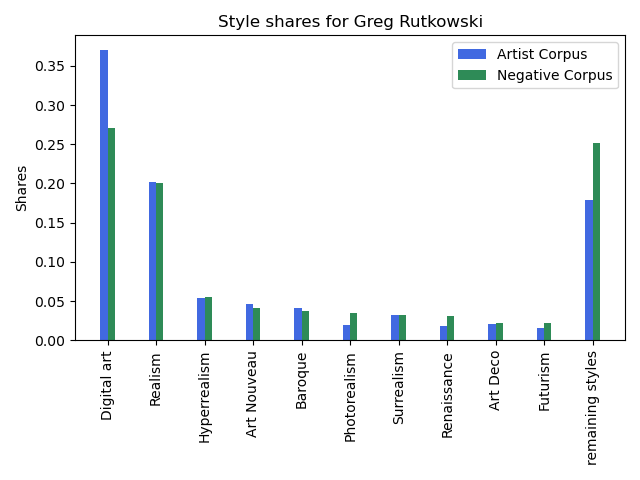
\includegraphics[height=7cm]{Bilder/style_proportions_example.png}\\[2.5ex]
    \end{center}
\caption{Example Style distribution for the 10 most popular styles and remaining styles}
\end{figure}


\section{Comparing Style distributions}

Artists with similar corpus and negative corpus have a smaller influence on the prompts they are used in. These artists are independent of the styles mentioned in the prompts.
I use the Bray-Curtis dissimilarity to evaluate the similarity between the two corpora. 
With these dissimilarity values, we can examine if there is a relation between the popularity of an artist and the artist's independence of the styles mentioned in the prompts.


\subsection{Bray-Curtis dissimilarity}

% stackexchange question
% https://stats.stackexchange.com/questions/609149/similarity-measure-for-two-discrete-distributions-a-group-of-proportions

% Comparison metrics is scaled in 0 to 1....
 %Soerensen-Dice coefficient
% https://en.wikipedia.org/wiki/S%C3%B8rensen%E2%80%93Dice_coefficient

%DSC =Dice similarity coefficient

%\[ DSC = \frac{2|X \cap Y|}{|X| + |Y|}\]

%Since \(|X|\) and \(|Y|\) are always one, we can simplify the formula to:

%\[ DSC = |X \cap Y|\]

% It is easier to use and reference the Bray Curtis dissimilarity

For comparing the style distributions, I will use the Bray-Curtis dissimilarity. It comes from Biology and quantifies the compositional dissimilarity between two sites, based on counts. In this case, we are comparing the style distributions of the artist corpus \(i\) with the negative corpus \(j\). The dissimilarity value is 0 for identical distributions and 1 for distributions without common elements. It is defined as:

\[ BC_{ij} = 1 - \frac{2C_{ij}}{S_i + S_j}\]

Since we express the style mentions as proportions, the sizes \(S_i\) and \(S_j\) are always one. The forluma is simplified to:

\[ BC_{ij} = 1 - C_{ij} \]


\(C_{ij}\) is the sum of the lesser values for styles in common between the compared prompts:

\[ C_{ij} = \sum_{s \in Styles} min(i_s,j_s)\]

Figure \ref{fig:dissimilarity_calculation_example} shows the calculation of a dissimilarity value. The red bars represent the shares \(min(i_s,j_s)\), that the style distributions of the artist corpus and negative corpus have in common. The summation of all the red bars equates to \(C_{ij}\). 

\begin{figure}[h]
    \begin{center}
        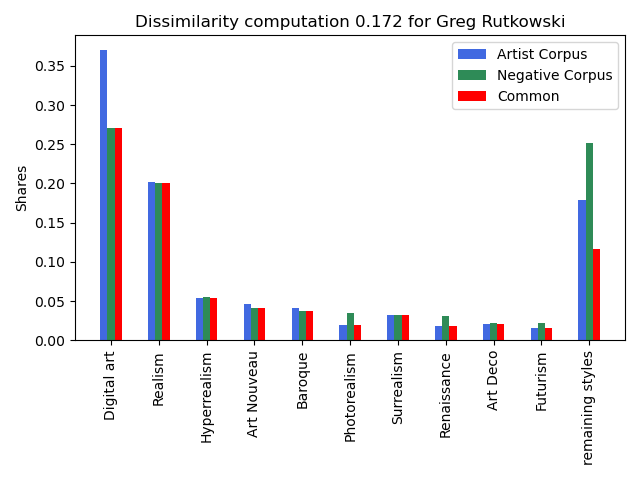
\includegraphics[height=7cm]{Bilder/dissimilarity_calculation_example.png}\\[2.5ex]
    \end{center}
\caption{Example Dissimilarity calculation}
\label{fig:dissimilarity_calculation_example}
\end{figure}



\subsection{Evaluating the observed dissimilarity}

The observed dissimilarity values will be analysed with Spearman's rank correlation coefficient. This correlation coefficient is chosen since it is appropriate for comparing two ranked variables and does not require the variables to satisfy conditions such as being normally distributed. In this case, the coefficient indicates whether the artist's popularity rank correlates with the style distributions' dissimilarity. The coefficient produces an \(r_s\) value between -1 and 1, where 1 indicates a perfect positive correlation, 0 indicates no correlation and -1 indicates a perfect negative correlation.

To check the significance of the correlation, we will use the \(p\) value of the Spearman's rank correlation coefficient. This \(p\) value is for a hypothesis test, where the null hypothesis states that the two variables are not correlated.

% The observed dissimilarity values will be visualized as well.




% if the p value is small, we have to reject the null hypothesis


\chapter{Results}
\label{cha:Results}
% \lipsum \autocite{DBLP:books/sp/HarderR01}
Results


TODO:

By using your method on your data, you will produce some
results (numbers, plots, etc.). Please note that any scripts
you will generate during the project should also be briefly
mentioned in the documentation. However, please do not
put source code in the documentation. Rather share with
us any scripts (and datasets) you create by means of a
repository.

\include{Inhalt/Conclusion}

%\include{Inhalt/Grundlagen...}

% Literaturverzeichnis -----------------------------------------------------
%		Das Literaturverzeichnis wird aus der Datenbank erstellt.
%		Die genaue Verwendung von biblatex wird hier jedoch nicht erklärt.
%		Links: 	https://ctan.org/pkg/biblatex?lang=de
%						https://de.overleaf.com/learn/latex/Articles/Getting_started_with_BibLaTeX
% --------------------------------------------------------------------------

\printbibliography

% \setcounter{page}{122}
% \pagenumbering{gobble}
%\pagenumbering{gobble}
\addchap{Erklärung}
Ich versichere, dass ich die vorliegende Arbeit mit dem Thema:

\begin{center}
\textit{\glqq\titel\grqq}\\[1em]
\end{center}
			
selbständig und nur unter Verwendung der angegebenen Quellen und Hilfsmittel angefertigt habe, insbesondere sind wörtliche oder sinngemäße Zitate als solche gekennzeichnet. Mir ist bekannt, dass Zuwiderhandlung auch nachträglich zur Aberkennung des Abschlusses führen kann.
\par
\ort, den \eingereicht


\rule[-0.2cm]{5cm}{0.5pt}

\textsc{\autor} 
	% Selbständigkeitserklärung 

\include{Inhalt/Arbeitsteilung}

% Anhang -------------------------------------------------------------------
%		Die Inhalte des Anhangs werden analog zu den Kapiteln inkludiert.
%		Dies geschieht in der Datei Anhang.tex
% --------------------------------------------------------------------------
\appendix
\clearpage
\renewcommand*{\thesection}{\Alph{section}} 
\pagenumbering{Roman}
%\include{Inhalt/Anhang}



% Index --------------------------------------------------------------------
%		Zum Erstellen eines Index, die folgende Zeile auskommentieren.
% --------------------------------------------------------------------------
%\printindex		% Index hier einfügen
%\ofoot{}
%\include{Inhalt/Thesen}	% Thesen 

\end{document}
